%---------------------------------------------------------------------------%
%-                                                                         -%
%-                           LaTeX Template                                -%
%-                                                                         -%
%---------------------------------------------------------------------------%
%- Copyright (C) Huangrui Mo <huangrui.mo@gmail.com> 
%- This is free software: you can redistribute it and/or modify it
%- under the terms of the GNU General Public License as published by
%- the Free Software Foundation, either version 3 of the License, or
%- (at your option) any later version.
%---------------------------------------------------------------------------%
%->> Document class declaration
%---------------------------------------------------------------------------%
\documentclass[singlesided]{Style/ucasthesis}%
%- Multiple optional arguments:
%- [<singlesided|doublesided|printcopy>]% set one or two sided eprint or print
%- [draftversion]% show draft version information
%- [fontset=<fandol|...>]% specify font set to replace automatic detection
%- [scheme=plain]% thesis writing of international students
%- [standard options for ctex book class: draft|paper size|font size|...]%
%---------------------------------------------------------------------------%
%->> Document settings
%---------------------------------------------------------------------------%
\usepackage[super,myhdr,list]{Style/artratex}% document settings
%- usage: \usepackage[option1,option2,...,optionN]{artratex}
%- Multiple optional arguments:
%- [bibtex|biber]% set bibliography processor and package
%- [<numbers|super|authoryear|alpha>]% set citation and reference style
%- <numbers>: textual: Jones [1]; parenthetical: [1]
%- <super>: textual: Jones superscript [1]; parenthetical: superscript [1]
%- <authoryear>: textual: Jones (1995); parenthetical: (Jones, 1995)
%- <alpha>: textual: not available; parenthetical: [Jon95]
%- [geometry]% reconfigure page layout via geometry package
%- [lscape]% provide landscape layout environment
%- [myhdr]% enable header and footer via fancyhdr package
%- [color]% provide color support via xcolor package
%- [background]% enable page background
%- [tikz]% provide complex diagrams via tikz package
%- [table]% provide complex tables via ctable package
%- [list]% provide enhanced list environments for algorithm and coding
%- [math]% enable some extra math packages
\usepackage{Style/artracom}% user defined commands

\let\openbox\relax
\usepackage{amsthm}

%---------------------------------------------------------------------------%
%->> 对于数学定理的表示
\theoremstyle{plain}
\newtheorem{thm}{定理}[section]
\newtheorem{lem}[thm]{引理}
\newtheorem{prop}[thm]{命题}
\newtheorem{cor}{推论}

\theoremstyle{definition}
\newtheorem{defn}{定义}[section]
\newtheorem{conj}{猜想}[section]
\newtheorem{exmp}{示例}[section]

\theoremstyle{remark}
\newtheorem*{rem}{标注}
\newtheorem*{note}{注解}

\newenvironment{pf}{{\noindent\it 证明.}\quad}{\hfill $\square$\par}
%---------------------------------------------------------------------------%
%->> Document inclusion
%---------------------------------------------------------------------------%
%\includeonly{Tex/Chap_1,...,Tex/Chap_N}% selected files compilation
%---------------------------------------------------------------------------%
%->> Document content
%---------------------------------------------------------------------------%
%===========================================================================%
%===========================================================================%
%    特别提醒:																%
%		参考文献需要严格按标准格式来写,常用的为J和C两类:                       %
%		J代表Journal论文,C代表Conference论文		                         %
%===========================================================================%
\begin{document}
	%-
	%-> Frontmatter: title page, abstract, content list, symbol list, preface
	%-
	\frontmatter% initialize the environment
	%---------------------------------------------------------------------------%
%->> 封面信息及生成
%---------------------------------------------------------------------------%
%-
%-> 中文封面信息
%-
\confidential{}% 密级:只有涉密论文才填写
\schoollogo{scale=0.2}{ShanghaiTechLogo}% 校徽
%======论文题目 页眉显示 务必准确========
\title{功能性脑类器官的工程化构建}% 论文中文题目
\author{唐林峥、虞果、刘思昀}% 论文作者
\ID{2022533087、2022533174、2022522011}
\entranceYear{2022}
\advisor{张寒}% 指导教师:姓名
\advisorsec{}% 第二指导老师:按情况填写
\degree{学士}% 学位:学士、硕士、博士
\degreetype{理学}% 学位类别:理学、工学、工程、医学等
\major{脑科学与脑疾病}% 二级学科专业名称
\institute{生物医学工程学院}% 院系名称
\chinesedate{二零二五年~一月}% 毕业日期:夏季为6月、冬季为12月
%-
%-> 英文封面信息
%-
\englishtitle{Engineering Functional Brain Organoids}% 论文英文题目
\englishauthor{Lin-Zheng Tang, Guo Yu, Si-Yun Liu}% 论文作者
\englishadvisor{Han Zhang}% 指导教师
\englishdegree{Bachelor}% 学位:Bachelor, Master, Doctor。封面格式将根据英文学位名称自动切换,请确保拼写准确无误
\englishdegreetype{Natural Science}% 学位类别:Philosophy, Natural Science, Engineering, Economics, Agriculture 等
\englishthesistype{thesis}% 论文类型: thesis, dissertation
\englishmajor{Brain Science and Brain Disorders}% 二级学科专业名称
\englishinstitute{School of Biomedical Engineering}% 院系名称
\englishdate{January 2025}% 毕业日期:夏季为June、冬季为December
%-
%-> 生成封面
%-
%-======================================================
% 封面和声明页格式不符合教务处要求,因此此处不生成pdf格式的 ||
% 论文封面和声明页,请各位使用word模板中的相关内容。       ||
%=======================================================
\maketitle% 生成中文封面
\makeenglishtitle% 生成英文封面
%-

\chapter*{摘\quad 要}\chaptermark{摘\quad 要}% 摘要标题
\setcounter{page}{1}% 开始页码
\pagenumbering{Roman}% 页码符号

本文探讨了基于自由能原理(Free Energy Principle, FEP)的智能脑类器官开发方法,旨在通过体外培养功能性神经网络来模拟人类大脑的发育和功能。脑类器官作为一种人工培养的组织,能够在实验室环境中模拟特定脑区的结构和功能,为研究神经系统疾病提供了新的实验平台。本文首先介绍了脑类器官的基本概念及其在神经科学研究中的重要性,随后详细阐述了自由能原理的理论框架及其在脑类器官训练中的应用。通过结合电刺激和化学刺激,本文提出了一种创新的脑类器官训练方法,并设计了一个基于海马体脑类器官的抑郁症模型。该模型不仅为抑郁症的机制研究提供了新的实验平台,还可用于药物筛选和网络水平变化的研究。

\keywords{脑类器官,自由能原理,神经网络,抑郁症模型,药物筛选}% 中文关键词

%-
%-> 英文摘要
%-
\chapter*{Abstract}\chaptermark{Abstract}% 摘要标题

This paper explores the development of intelligent brain organoids based on the Free Energy Principle (FEP), aiming to simulate the development and functionality of the human brain by cultivating functional neural networks in vitro. Brain organoids, as artificially grown tissues, can mimic the structure and function of specific brain regions in a laboratory setting, providing a novel experimental platform for studying neurological disorders. The paper begins by introducing the basic concepts of brain organoids and their significance in neuroscience research. It then elaborates on the theoretical framework of the Free Energy Principle and its application in training brain organoids. By combining electrical and chemical stimuli, this paper proposes an innovative method for training brain organoids and designs a depression model based on hippocampal organoids. This model not only offers a new experimental platform for studying the mechanisms of depression but also facilitates drug screening and research on network-level changes.

\englishkeywords{Brain Organoids, Free Energy Principle, Neural Networks, Depression Model, Drug Screening}% 英文关键词
%---------------------------------------------------------------------------%
% title page, abstract, dedication
	{% content list region
		\linespread{1.2}% local line space
		%\intotoc{\contentsname}% add link to contents table and bookmark
		\tableofcontents% contents catalog
		%\intotoc{\listfigurename}% add link to contents table and bookmark
		%\listoffigures% figures catalog
		%\intotoc{\listtablename}% add link to contents table and bookmark
		%\listoftables% tables catalog
	}
	% \chapter*{符号列表}
\chaptermark{符号列表}

\section*{字符}
\nomenclatureitem[\textbf{Unit}]{\textbf{Symbol}}{\textbf{Description}}
\nomenclatureitem[$\Unit{m^{2} \cdot s^{-2} \cdot K^{-1}}$]{$R$}{the gas constant}
\nomenclatureitem[$\Unit{m^{2} \cdot s^{-2} \cdot K^{-1}}$]{$C_v$}{specific heat capacity at constant volume}
\nomenclatureitem[$\Unit{m^{2} \cdot s^{-2} \cdot K^{-1}}$]{$C_p$}{specific heat capacity at constant pressure}
\nomenclatureitem[$\Unit{m^{2} \cdot s^{-2}}$]{$E$}{specific total energy}
\nomenclatureitem[$\Unit{m^{2} \cdot s^{-2}}$]{$e$}{specific internal energy}
\nomenclatureitem[$\Unit{m^{2} \cdot s^{-2}}$]{$h_T$}{specific total enthalpy}
\nomenclatureitem[$\Unit{m^{2} \cdot s^{-2}}$]{$h$}{specific enthalpy}
\nomenclatureitem[$\Unit{kg \cdot m \cdot s^{-3} \cdot K^{-1}}$]{$k$}{thermal conductivity}
\nomenclatureitem[$\Unit{kg \cdot m^{-1} \cdot s^{-2}}$]{$S_{ij}$}{deviatoric stress tensor}
\nomenclatureitem[$\Unit{kg \cdot m^{-1} \cdot s^{-2}}$]{$\tau_{ij}$}{viscous stress tensor}
\nomenclatureitem[$\Unit{1}$]{$\delta_{ij}$}{Kronecker tensor}
\nomenclatureitem[$\Unit{1}$]{$I_{ij}$}{identity tensor}

\section*{算子}
\nomenclatureitem{\textbf{Symbol}}{\textbf{Description}}
\nomenclatureitem{$\Delta$}{difference}
\nomenclatureitem{$\nabla$}{gradient operator}
\nomenclatureitem{$\delta^{\pm}$}{upwind-biased interpolation scheme}

\section*{缩写}
\nomenclatureitem{CFD}{Computational Fluid Dynamics}
\nomenclatureitem{CFL}{Courant-Friedrichs-Lewy}
\nomenclatureitem{EOS}{Equation of State}
\nomenclatureitem{JWL}{Jones-Wilkins-Lee}
\nomenclatureitem{WENO}{Weighted Essentially Non-oscillatory}
\nomenclatureitem{ZND}{Zel'dovich-von Neumann-Doering}

% list of symbols, preface content
	%-
	%-> Mainmatter
	%-
	\mainmatter% initialize the environment
	%---------------------------------------------------------------------------%
%->> Main content
%---------------------------------------------------------------------------%
\chapter{引言}\label{chap:introduction}

\section{脑类器官的理解}\label{sec:brain-organoid}
脑类器官是一种在体外人工培养的组织,其形态和功能类似于人类大脑的某些部分\cite{Kim2023}。
通过干细胞技术,科学家能够在实验室中培养出这些微型脑组织,用于研究大脑发育、疾病机制以及药物筛选等领域。
脑类器官的出现为神经科学研究提供了一个高度可控的实验平台,尤其是在研究复杂神经系统疾病时,其优势尤为明显。


\section{研究目的}\label{sec:research-purpose}
脑类器官的主要目的是在更加可控的环境中研究与大脑相关的疾病。
传统的动物模型虽然在一定程度上能够模拟人类大脑的功能,但由于物种差异,其研究结果往往难以直接应用于人类。
而脑类器官则能够更好地模拟人类大脑的发育和功能,为研究神经系统疾病提供了新的可能性。


\section{面临的挑战}\label{sec:research-challenges}
尽管脑类器官在研究中展现出巨大的潜力,但其发展仍面临诸多挑战。
首先,从物理结构上来看,脑类器官的构建非常复杂。
大脑是一个高度复杂的器官,包含多个功能区域和复杂的血管结构,因此用现有技术培养一个真实比例的体外大脑的成本几乎是不可接受的;其次,从功能角度来看,脑类器官的功能发育也面临挑战。
即使能够构建出形态上相似的脑类器官,如何使其具备与真实大脑相似的神经元网络,以具备相似的功能,仍然是一个重要的研究方向。


\section{可能的解决方案}\label{sec:research-solutions}
针对上述挑战,研究者提出了两种可能的解决方案。
首先,从物理结构的角度,可以通过专注于重建特定的大脑区域来简化问题。
例如,选择重建海马体或前额叶皮层等特定区域,而不是试图重建整个大脑。
其次,从功能发育的角度,可以通过主动“训练”脑类器官,使其接受类似于真实大脑的完整刺激,从而促进其功能发育。
这种训练可以通过电刺激、化学刺激或光遗传学等手段实现。



\chapter{背景}\label{chap:background}

\section{特定脑区的重建}\label{sec:brain-region-reconstruction}
在脑类器官的研究中,重建特定脑区是一个重要的研究方向\cite{Kim2023}。已有大量研究专注于如何通过干细胞技术培养出特定脑区的类器官。例如,海马体、前额叶皮层和小脑等区域的重建已经取得了显著进展。这些研究为脑类器官的功能研究提供了重要的基础。

\section{自由能原理}\label{sec:free-energy-principle}
自由能原理(Free Energy Principle, FEP)是由 Karl Friston 于 2010 年提出的一种关于生命体智能的规范性理论\cite{Friston2010}。该理论基于变分贝叶斯推断,认为生命体通过最小化自由能(即“惊奇”)来维持其内部状态与外部环境的一致性。自由能原理为理解大脑如何通过学习和适应来应对外部环境提供了理论框架。

\section{自由能原理的数学表达}\label{sec:free-energy-math}
自由能原理的核心思想可以通过以下数学公式表达:

\[
F(\mu, a; s) = \mathbb{E}_{q(\psi)} \left[ -\log p(\psi, s, a, \mu \mid \psi) \right] - \mathcal{H}[q(\psi \mid s, a, \mu, \psi)]
\]

其中,$F(\mu, a; s)$ 表示自由能,$\mathbb{E}_{q(\psi)}$ 表示期望能量,$\mathcal{H}$ 表示熵。自由能原理认为,大脑通过变分贝叶斯推断来最小化自由能,从而使其对外部环境的预测尽可能准确。

\section{盘中之脑}\label{sec:dish-brain}
自由能原理不仅在理论上具有重要意义,还在实际研究中得到了广泛应用。例如,基于自由能原理的“培养皿大脑”(Dish Brain)项目成功训练了一个神经网络来玩电子游戏\cite{Kagan2022}。这一研究表明,通过外部刺激和奖励机制,可以在体外培养出具有学习能力的神经网络。


\chapter{方法论}\label{chap:methodlogy}

\chapter{具体设计样例}\label{chap:design}

\section{抑郁症模型的需求}\label{sec:depression-model-requirement}
抑郁症是一种复杂的神经系统疾病,涉及神经和生化过程的多种紊乱。
尽管已有大量研究致力于抑郁症的机制研究,但现有的动物模型仍存在诸多争议。
脑类器官为抑郁症的研究提供了一个新的实验平台,能够更好地模拟人类大脑的功能和病理变化。

\begin{figure}[!htbp]
    \centering
    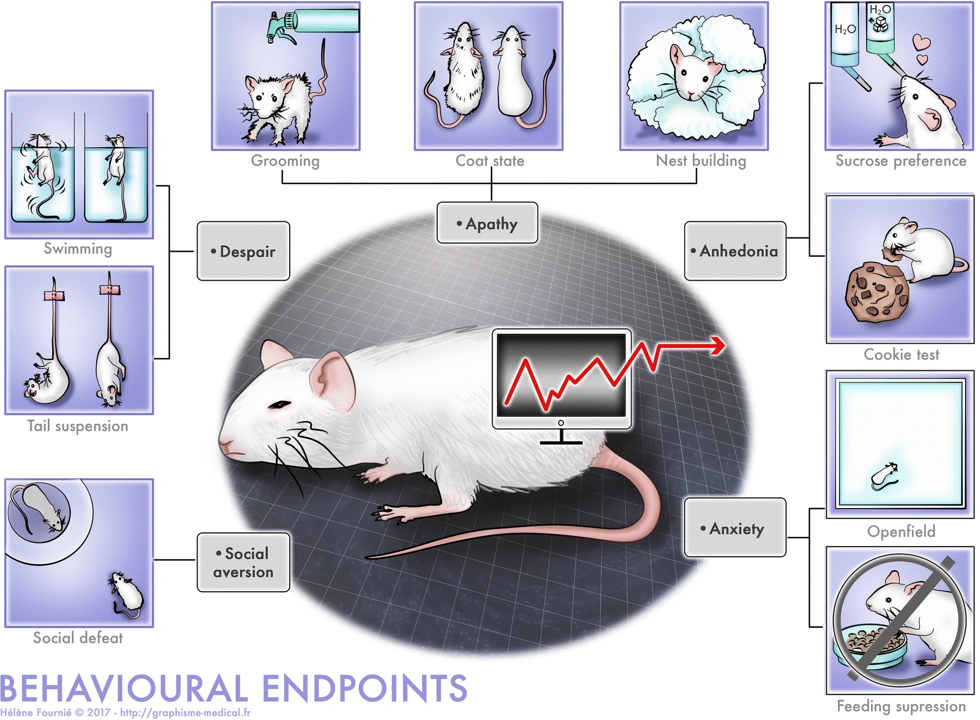
\includegraphics[width=0.75\textwidth]{Img/depression-model.png}
    \bicaption{现有的抑郁症动物模型示意图}{Existing Animal Models of Depression}
    \label{fig:depression-model}
\end{figure}

\section{研究目标}\label{sec:research-objective}
本研究的目标是通过结合电刺激和化学刺激,训练出一个功能性的健康海马体脑类器官。
在此基础上,引入常见的抑郁症诱导机制,如毒性化合物和电刺激,诱导海马体脑类器官进入疾病状态。
这一研究将为抑郁症的机制研究和药物筛选提供新的实验模型。


\section{实验设计}\label{sec:experiment-design}
\subsection{宏观培养}\label{subsec:macro-culture}
首先,将 hiPSC 分化为海马体神经元,并直接在微电极阵列(MEA)芯片上进行培养。
通过精确控制培养条件,确保海马体脑类器官的形态和功能与真实大脑相似。

\begin{figure}[!htbp]
    \centering
    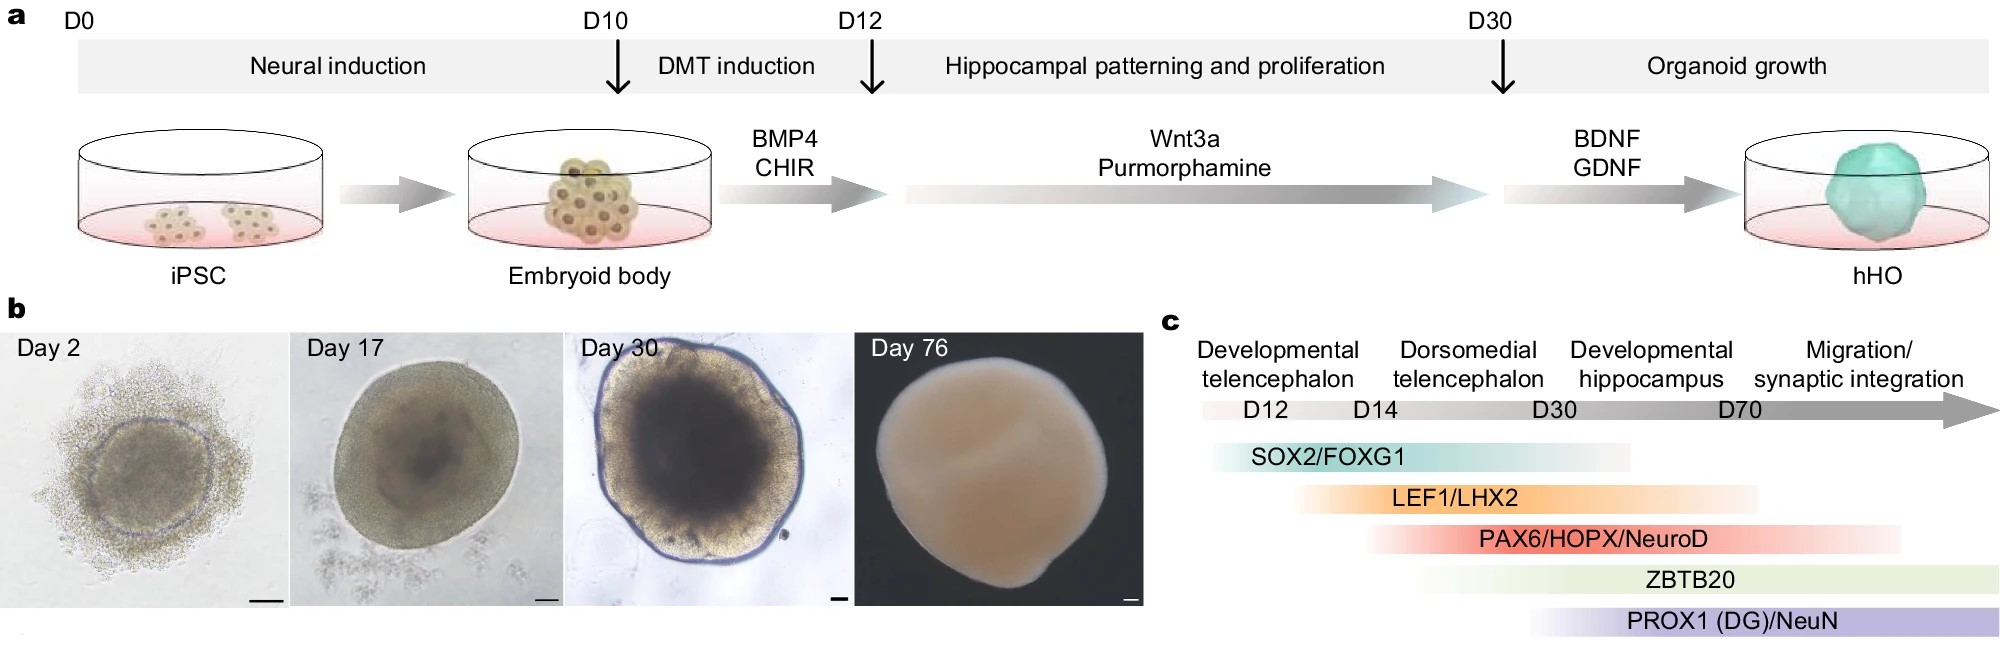
\includegraphics[width=0.75\textwidth]{Img/hipp-organoid.jpg}
    \bicaption{海马体脑类器官的培养示意图}{Schematic Diagram of Hippocampal Organoid}
    \label{fig:hipp-organoid}
\end{figure}

\subsection{微观培养}\label{subsec:micro-culture}
在微观培养阶段,通过外部刺激作为奖励或惩罚信号,训练海马体脑类器官的神经网络。
这一过程将帮助脑类器官形成功能性的神经网络,并模拟真实大脑的学习过程。

\begin{figure}[!htbp]
    \centering
    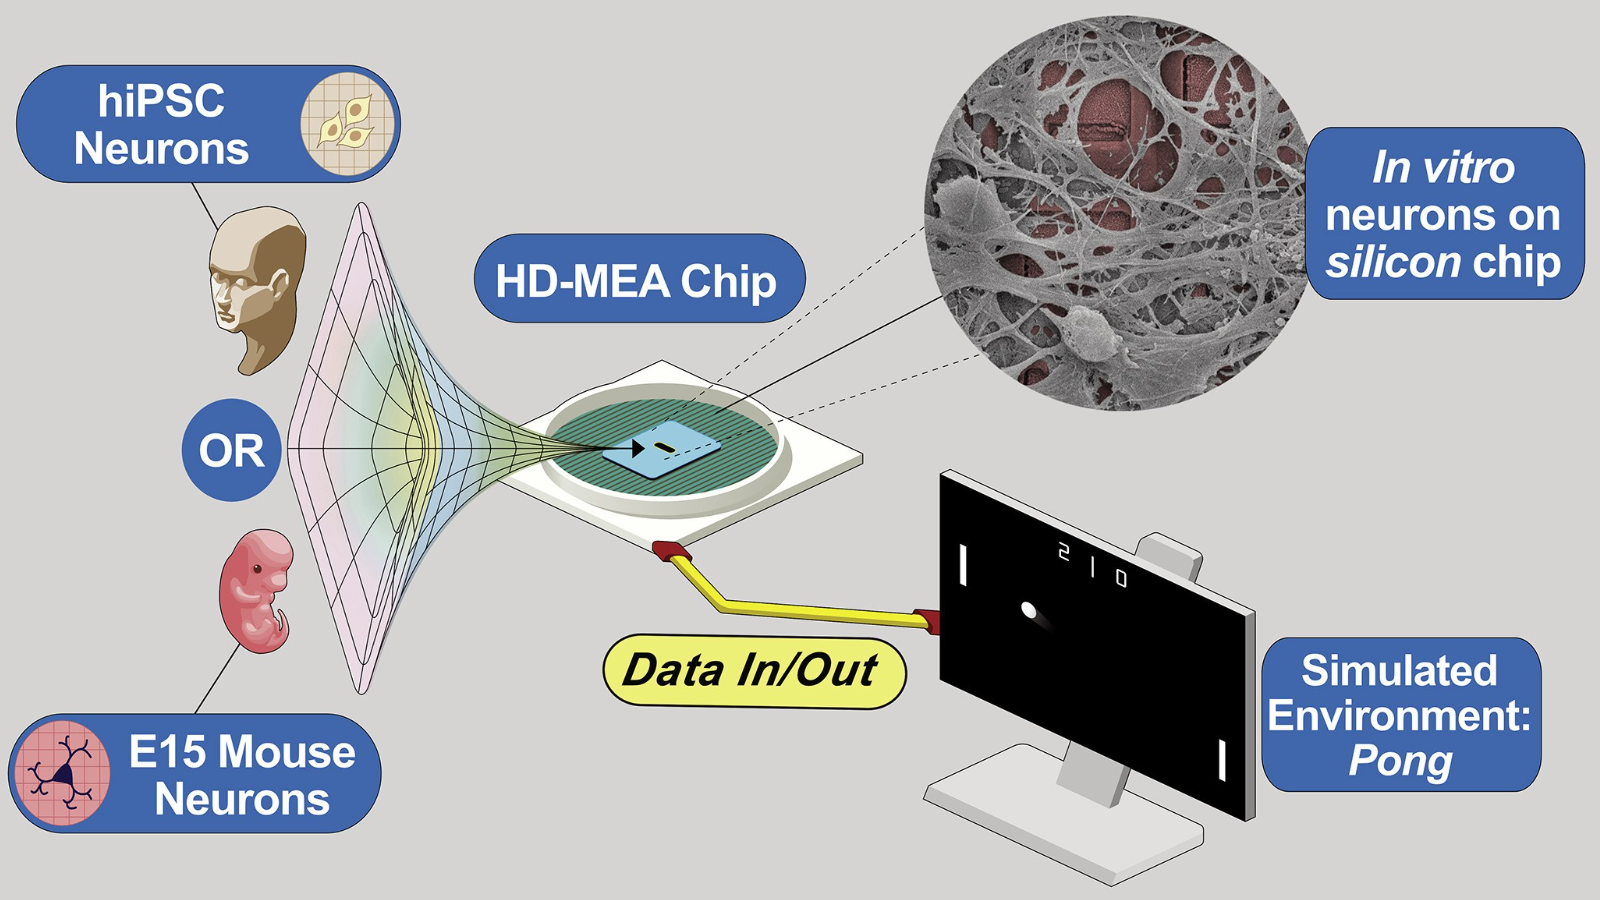
\includegraphics[width=0.75\textwidth]{Img/demo-dishbarin.png}
    \bicaption{盘中之脑的训练设计}{Training Design of Dish Brain}
    \label{fig:demo-dishbarin}
\end{figure}

\subsection{抑郁症诱导}\label{subsec:depression-induction}
在脑类器官形成功能性神经网络后,引入抑郁症诱导机制。
通过使用皮质酮、IL-6 和 TNF-α 等化学物质,以及电刺激,诱导海马体脑类器官进入疾病状态。
这一过程将模拟抑郁症的病理变化,为研究抑郁症的机制提供新的实验平台。


\section{应用前景}\label{sec:application-prospect}
本研究提出的抑郁症模型具有广泛的应用前景。
首先,它为抑郁症的机制研究提供了一个创新的实验平台。
其次,该模型可以用于药物筛选,帮助开发新的抗抑郁药物。
最后,通过研究脑类器官在疾病状态下的网络水平变化,可以为理解精神健康障碍提供新的见解。



%---------------------------------------------------------------------------%
% main content
	% %-
	% %-> Appendix
	% %-
	% \cleardoublepage%
	% \appendix% initialize the environment
	% \chapter{中国科学院大学学位论文撰写要求}

学位论文是研究生科研工作成果的集中体现,是评判学位申请者学术水平、授予其学位的主要依据,是科研领域重要的文献资料。根据《科学技术报告、学位论文和学术论文的编写格式》(GB/T 7713-1987)、《学位论文编写规则》(GB/T 7713.1-2006)和《文后参考文献著录规则》(GB7714—87)等国家有关标准,结合中国科学院大学(以下简称“国科大”)的实际情况,特制订本规定。

\section{论文无附录者无需附录部分}

\section{测试公式编号} \label{sec:testmath}

\begin{equation} \label{eq:appedns}
    \begin{cases}
        \frac{\partial \rho}{\partial t} + \nabla\cdot(\rho\Vector{V}) = 0 \ \mathrm{times\ font\ test}\\
        \frac{\partial (\rho\Vector{V})}{\partial t} + \nabla\cdot(\rho\Vector{V}\Vector{V}) = \nabla\cdot\Tensor{\sigma} \ \text{times font test}\\
        \frac{\partial (\rho E)}{\partial t} + \nabla\cdot(\rho E\Vector{V}) = \nabla\cdot(k\nabla T) + \nabla\cdot(\Tensor{\sigma}\cdot\Vector{V})
    \end{cases}
\end{equation}
\begin{equation}
    \frac{\partial }{\partial t}\int\limits_{\Omega} u \, \mathrm{d}\Omega + \int\limits_{S} \unitVector{n}\cdot(u\Vector{V}) \, \mathrm{d}S = \dot{\phi}
\end{equation}

\section{测试生僻字}

霜蟾盥薇曜灵霜颸妙鬘虚霩淩澌菀枯菡萏泬寥窅冥毰毸濩落霅霅便嬛岧峣瀺灂姽婳愔嫕飒纚棽俪緸冤莩甲摛藻卮言倥侗椒觞期颐夜阑彬蔚倥偬澄廓簪缨陟遐迤逦缥缃鹣鲽憯懔闺闼璀错媕婀噌吰澒洞阛闠覼缕玓瓑逡巡諓諓琭琭瀌瀌踽踽叆叇氤氲瓠犀流眄蹀躞赟嬛茕頔璎珞螓首蘅皋惏悷缱绻昶皴皱颟顸愀然菡萏卑陬纯懿犇麤掱暒 墌墍墎墏墐墒墒墓墔墕墖墘墖墚墛坠墝增墠墡墢墣墤墥墦墧墨墩墪樽墬墭堕墯墰墱墲坟墴墵垯墷墸墹墺墙墼墽垦墿壀壁壂壃壄壅壆坛壈壉壊垱壌壍埙壏壐壑壒压壔壕壖壗垒圹垆壛壜壝垄壠壡坜壣壤壥壦壧壨坝塆圭嫶嫷嫸嫹嫺娴嫼嫽嫾婳妫嬁嬂嬃嬄嬅嬆嬇娆嬉嬊娇嬍嬎嬏嬐嬑嬒嬓嬔嬕嬖嬗嬘嫱嬚嬛嬜嬞嬟嬠嫒嬢嬣嬥嬦嬧嬨嬩嫔嬫嬬奶嬬嬮嬯婴嬱嬲嬳嬴嬵嬶嬷婶嬹嬺嬻嬼嬽嬾嬿孀孁孂娘孄孅孆孇孆孈孉孊娈孋孊孍孎孏嫫婿媚嵭嵮嵯嵰嵱嵲嵳嵴嵵嵶嵷嵸嵹嵺嵻嵼嵽嵾嵿嶀嵝嶂嶃崭嶅嶆岖嶈嶉嶊嶋嶌嶍嶎嶏嶐嶑嶒嶓嵚嶕嶖嶘嶙嶚嶛嶜嶝嶞嶟峤嶡峣嶣嶤嶥嶦峄峃嶩嶪嶫嶬嶭崄嶯嶰嶱嶲嶳岙嶵嶶嶷嵘嶹岭嶻屿岳帋巀巁巂巃巄巅巆巇巈巉巊岿巌巍巎巏巐巑峦巓巅巕岩巗巘巙巚帠帡帢帣帤帨帩帪帬帯帰帱帲帴帵帷帹帺帻帼帽帾帿幁幂帏幄幅幆幇幈幉幊幋幌幍幎幏幐幑幒幓幖幙幚幛幜幝幞帜幠幡幢幤幥幦幧幨幩幪幭幮幯幰幱庍庎庑庖庘庛庝庠庡庢庣庤庥庨庩庪庬庮庯庰庱庲庳庴庵庹庺庻庼庽庿廀厕廃厩廅廆廇廋廌廍庼廏廐廑廒廔廕廖廗廘廙廛廜廞庑廤廥廦廧廨廭廮廯廰痈廲廵廸廹廻廼廽廿弁弅弆弇弉弖弙弚弜弝弞弡弢弣弤弨弩弪弫弬弭弮弰弲弪弴弶弸弻弼弽弿彖彗彘彚彛彜彝彞彟彴彵彶彷彸役彺彻彽彾佛徂徃徆徇徉后徍徎徏径徒従徔徕徖徙徚徛徜徝从徟徕御徢徣徤徥徦徧徨复循徫旁徭微徯徰徱徲徳徴徵徶德徸彻徺忁忂惔愔忇忈忉忔忕忖忚忛応忝忞忟忪挣挦挧挨挩挪挫挬挭挮挰掇授掉掊掋掍掎掐掑排掓掔掕挜掚挂掜掝掞掟掠采探掣掤掦措掫掬掭掮掯掰掱掲掳掴掵掶掸掹掺掻掼掽掾掿拣揁揂揃揅揄揆揇揈揉揊揋揌揍揎揑揓揔揕揖揗揘揙揤揥揦揧揨揫捂揰揱揲揳援揵揶揷揸揻揼揾揿搀搁搂搃搄搅搇搈搉搊搋搌搎搏搐搑搒摓摔摕摖摗摙摚摛掼摝摞摠摡斫斩斮斱斲斳斴斵斶斸旪旫旮旯晒晓晔晕晖晗晘晙晛晜晞晟晠晡晰晣晤晥晦晧晪晫晬晭晰晱晲晳晴晵晷晸晹晻晼晽晾晿暀暁暂暃暄暅暆暇晕晖暊暋暌暍暎暏暐暑暒暓暔暕暖暗旸暙暚暛暜暝暞暟暠暡暣暤暥暦暧暨暩暪暬暭暮暯暰昵暲暳暴暵暶暷暸暹暺暻暼暽暾暿曀曁曂曃晔曅曈曊曋曌曍曎曏曐曑曒曓曔曕曗曘曙曚曛曜曝曞曟旷曡曢曣曤曥曦曧昽曩曪曫晒曭曮曯椗椘椙椚椛検椝椞椟椠椡椢椣椤椥椦椧椨椩椪椫椬椭椮椯椰椱椲椳椴椵椶椷椸椹椺椻椼椽椾椿楀楁楂楃楅楆楇楈楉杨楋楌楍榴榵榶榷榸榹榺榻榼榽榾桤槀槁槂盘槄槅槆槇槈槉槊构槌枪槎槏槐槑槒杠槔槕槖槗滙滛滜滝滞滟滠滢滣滦滧滪滫沪滭滮滰滱渗滳滵滶滹滺浐滼滽漀漃漄漅漈漉溇漋漌漍漎漐漑澙熹漗漘漙沤漛漜漝漞漟漡漤漥漦漧漨漪渍漭漮漯漰漱漳漴溆漶漷漹漺漻漼漽漾浆潀颍潂潃潄潅潆潇潈潉潊潋潌潍潎潏潐潒潓洁潕潖潗潘沩潚潜潝潞潟潠潡潢潣润潥潦潧潨潩潪潫潬潭浔溃潱潲潳潴潵潶滗潸潹潺潻潼潽潾涠澁澄澃澅浇涝澈澉澊澋澌澍澎澏湃澐澑澒澓澔澕澖涧澘澙澚澛澜澝澞澟渑澢澣泽浍澯澰淀澲澳澴澵澶澷澸潇潆瀡瀢瀣瀤瀥潴泷濑瀩瀪瀫瀬瀭瀮瀯弥瀱潋瀳瀴瀵瀶瀷瀸瀹瀺瀻瀼瀽澜瀿灀灁瀺灂沣滠灅灆灇灈灉灊灋灌灍灎灏灐洒灒灓漓灖灗滩灙灚灛灜灏灞灟灠灡灢湾滦灥灦灧灨灪燝燞燠燡燢燣燤燥灿燧燨燩燪燫燮燯燰燱燲燳烩燵燵燸燹燺薰燽焘燿爀爁爂爃爄爅爇爈爉爊爋爌烁爎爏爑爒爓爔爕爖爗爘爙爚烂爜爝爞爟爠爡爢爣爤爥爦爧爨爩猽猾獀犸獂獆獇獈獉獊獋獌獍獏獐獑獒獓獔獕獖獗獘獙獚獛獜獝獞獟獠獡獢獣獤獥獦獧獩狯猃獬獭狝獯狞獱獳獴獶獹獽獾獿猡玁玂玃。
% appendix content
	%-
	%-> Backmatter: bibliography, glossary, index
	%-
	\backmatter% initialize the environment
	\intotoc{\bibname}% add link to contents table and bookmark
	\bibliography{Biblio/ref}% bibliography
	% %\chapter{作者简历及攻读学位期间发表的学术论文与研究成果}
%
%\textbf{本科生无需此部分}。
%
%\section*{作者简历}
%
%\subsection*{casthesis作者}
%
%吴凌云,福建省屏南县人,中国科学院数学与系统科学研究院博士研究生。
%
%\subsection*{ucasthesis作者}
%
%莫晃锐,湖南省湘潭县人,中国科学院力学研究所硕士研究生。
%
%\section*{已发表(或正式接受)的学术论文:}
%
%[1] ucasthesis: A LaTeX Thesis Template for the University of Chinese Academy of Sciences, 2014.
%
%\section*{申请或已获得的专利:}
%
%(无专利时此项不必列出)
%
%\section*{参加的研究项目及获奖情况:}
%
%可以随意添加新的条目或是结构。

\chapter[致谢]{致\quad 谢}\chaptermark{致\quad 谢}% syntax: \chapter[目录]{标题}\chaptermark{页眉}
%\thispagestyle{noheaderstyle}% 如果需要移除当前页的页眉
%\pagestyle{noheaderstyle}% 如果需要移除整章的页眉
\pagestyle{mainmatterstyle} % 与前文页眉页脚格式相同

感激casthesis作者吴凌云学长,gbt7714-bibtex-style
开发者zepinglee,和ctex众多开发者们。若没有他们的辛勤付出和非凡工作,\LaTeX{}菜鸟的我是无法完成此国科大学位论文\LaTeX{}模板ucasthesis的。在\LaTeX{}中的一点一滴的成长源于开源社区的众多优秀资料和教程,在此对所有\LaTeX{}社区的贡献者表示感谢!

ucasthesis国科大学位论文\LaTeX{}模板的最终成型离不开以霍明虹老师和丁云云老师为代表的国科大学位办公室老师们制定的官方指导文件和众多ucasthesis用户的热心测试和耐心反馈,在此对他们的认真付出表示感谢。特别对国科大的赵永明同学的众多有效反馈意见和建议表示感谢,对国科大本科部的陆晴老师和本科部学位办的丁云云老师的细致审核和建议表示感谢。谢谢大家的共同努力和支持,让ucasthesis为国科大学子使用\LaTeX{}撰写学位论文提供便利和高效这一目标成为可能。

\cleardoublepage[plain]% 让文档总是结束于偶数页,可根据需要设定页眉页脚样式,如 [noheaderstyle]

% other information
\end{document}
%---------------------------------------------------------------------------%

